% VUT FIT MITAI
% MSZ 2021/2022
% Author: Vladimir Dusek
% Login: xdusek27

%%%%%%%%%%%%%%%%%%%%%%%%%%%%%%%%%%%%%%%%%%%%%%%%%%%%%%%%%%%%%%%%%%%%%%%%%%%%%%%%

% Path to figures
\graphicspath{{upa/postrelacni_a_rozsirene_relacni/figures}}

%%%%%%%%%%%%%%%%%%%%%%%%%%%%%%%%%%%%%%%%%%%%%%%%%%%%%%%%%%%%%%%%%%%%%%%%%%%%%%%%

\chapter{UPA~--~Postrelační a rozšířené relační databáze (objektový a objektově relační databázový model -- struktura a operace; podpora práce s XML a JSON dokumenty v databázích).}

%%%%%%%%%%%%%%%%%%%%%%%%%%%%%%%%%%%%%%%%%%%%%%%%%%%%%%%%%%%%%%%%%%%%%%%%%%%%%%%%

\section{Zdroje}

\begin{compactitem}
    \item \path{01-uvod.pdf}
    \item \path{02-ordbms.pdf}
    \item \path{szz-discord-bazi.pdf}
    \item \path{szz-kastak.pdf}
    \item \path{Wikipedia}
    \item Mé materiály k UPA.
\end{compactitem}

%%%%%%%%%%%%%%%%%%%%%%%%%%%%%%%%%%%%%%%%%%%%%%%%%%%%%%%%%%%%%%%%%%%%%%%%%%%%%%%%

\section{Úvod a kontext}

\begin{compactitem}
    \item Postrelační databázový systém je relační databázový systém rozšířený o určitou specifikaci na databázové úrovni, protože aplikační řešení problému by bylo nedostačující (neefektivní). \begin{compactitem}
        \item Na konci 80. let roste vliv objektové orientace. To má za důsledek vznik objektových databází a rozširování schopností relačních databází (SŘBD) nad rámec relačního modelu.
    \end{compactitem}
    \item Vývoj databází \begin{compactitem}
        \item Relační model, SŘBD, standard SQL.
        \item Objektově orientované SŘBD.
        \item Objektově relační DB, datové sklady, získávání znalostí z dat.
        \item NoSQL databáze, podpora XML a JSON, grafové databáze, BigData, Data Science.
    \end{compactitem}
\end{compactitem}

\subsection{Relační databáze}

\begin{compactitem}
    \item Datový model: \begin{compactitem}
        \item relační model dat;
        \item kolekce (normalizovaných) tabulek (relací);
        \item omezená množina datových typů (jednoduché datové typy, typicky pevné délky);
        \item vztahy mezi řádky tabulek ($1:N$) vyjádřeny pomocí cizích a kandidátních klíčů;
        \item pro vztahy $M:N$ je nutná vazební tabulka.
    \end{compactitem}

    \item Dotazovací jazyk:\begin{compactitem}
        \item deklarativní -- SQL (matematická logika).
    \end{compactitem}

    \item Výpočetní model: \begin{compactitem}
        \item založený na hodnotách ve sloupcích tabulek;
        \item žádné reference ani ukazatele;
        \item jednoduchá navigace pomocí kurzoru.
    \end{compactitem}

    \item Standardizováno (SQL 1986).
\end{compactitem}

\begin{figure}[H]
    \centering
    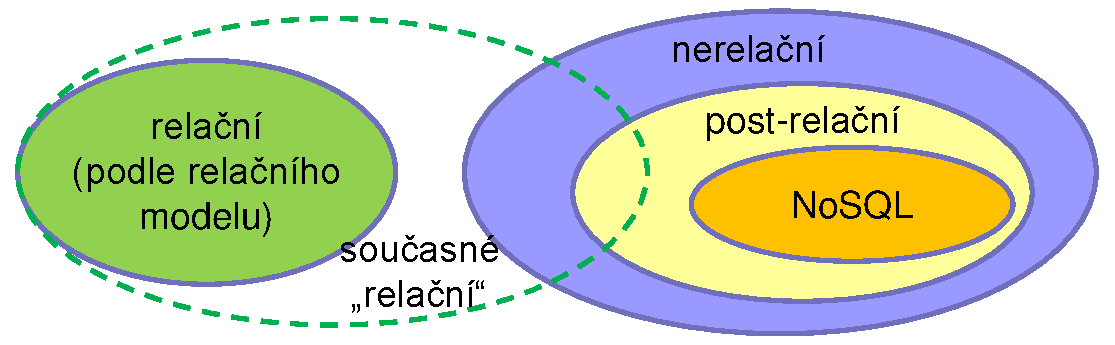
\includegraphics[width=1\linewidth]{postrelacni.pdf}
    \caption{Schéma databází.}
\end{figure}

%%%%%%%%%%%%%%%%%%%%%%%%%%%%%%%%%%%%%%%%%%%%%%%%%%%%%%%%%%%%%%%%%%%%%%%%%%%%%%%%

\section{Objektové databáze}

\begin{compactitem}
    \item Objektová databáze je databázový řízený systém, ve kterém je informace reprezentována ve formě objektů a používá se v objektově orientovaném programování.

    \item Umožňují modelování a vytváření perzistentních dat jako objektů.

    \item OSŘBD (Objektový systém řízení báze dat) musí splňovat kritéria ŠŘBD a musí to být OO systém.

    \item Objektové databáze nenahrazují, nýbrž doplňují relační (dnes spíše objektově-relační).

    \item Datový model: \begin{compactitem}
        \item Neexisuje jednoznačná definice jako u relačního modelu.
        \item Objektový (třídy, zapouzdření, dědičnost, polymorfismus, jednoznačný OID, komunikace zasílání zpráv).

        \item Databáze je tvořena kolekcí objektů, které mezi sebou komunikují zasíláním zpráv.

        \item Vlastnosti objektu jsou definovány třídou, ta zapouzdřuje data i chování.

        \item Data jsou reprezentovány atributy, chování je definováno metodami třídy.

        \item Atributy objektů mohou být jiné objekty (abstraktní datové typy).
        \item Vztahy objektů vytvářené pomocí referencí prostřednictvím OID.
        \item Vztahy $M:M$ lze vytvářet přímo.
    \end{compactitem}

    \item Dotazovací jazyk: \begin{compactitem}
        \item Object Query Langauge (OQL) -- snaha o vytvoření standardu jako obdoba SQL;
        \item Objektově orientované jazyky (typicky Java).
    \end{compactitem}

    \item Výpočetní model: \begin{compactitem}
        \item Navigace po objektové struktuře pomocí referencí prostřednictvím OID.
    \end{compactitem}

    \item Neexistuje standardizace.
\end{compactitem}

%%%%%%%%%%%%%%%%%%%%%%%%%%%%%%%%%%%%%%%%%%%%%%%%%%%%%%%%%%%%%%%%%%%%%%%%%%%%%%%%

\section{Objektově relační databáze}

\begin{compactitem}
    \item Objektově relační databáze je hybridem objektové a relační databáze. \begin{compactitem}
        \item Cílem je spojit výhody relačního a objektového modelu.
    \end{compactitem}

    \item Objektové rysy ve standardu SQL.
    \item První OSŘBD: PostreSQL (open source).
    \item Podpora objektových rozšíření u některých SŘBD (Oracle, IBM, \dots).

    \item Datový model: \begin{compactitem}
        \item Relační základ (tabulka) zůstává, ale jde o obecnější (vnořené) relace. Hodnoty mohou mít bohatší strukturu definovanou jako abstraktní datový typ (ADT).
        \item ADT zapouzdřuje data a operace.
        \item Podpora dědičnosti a polymorfismu.
        \item Zavedena obdoba OID, která umožňuje vytvářet nový typ vazeb mezi tabulkami.
        \item Nesplňuje normalizaci relační databáze.
    \end{compactitem}

    \item Dotazovací jazyk: \begin{compactitem}
        \item dialekt SQL (objektové rozšíření).
    \end{compactitem}

    \item Výpočetní model: \begin{compactitem}
        \item navigace po tabulkách pomocí kurzoru i pomocí reference.
    \end{compactitem}

    \item Standardizováno (SQL 1999).

    \item Objektově relační rysy: \begin{compactitem}
        \item Objektový model je založený na konceptech. \begin{compactitem}
            \item Strukturovaný datový typ.
            \item Typová tabulka.
        \end{compactitem}
        \item Uživatelem definované typy (UDT). \begin{compactitem}
            \item Odpovídají abstraktním datovým typům.
        \end{compactitem}
    \end{compactitem}
\end{compactitem}

%%%%%%%%%%%%%%%%%%%%%%%%%%%%%%%%%%%%%%%%%%%%%%%%%%%%%%%%%%%%%%%%%%%%%%%%%%%%%%%%

\section{Objektově relační mapování}

\begin{compactitem}
    \item Objektově relační mapování slouží k odstranění sémantické \uv{mezery} mezi OO modelem aplikací v OO jazyce a relačním databázovým modelem.
    \begin{compactitem}
        \item Zajišťuje automatickou konverzi dat mezi relační databází a objektově orientovaným programovacím jazykem.
    \end{compactitem}

    \item Zajišťuje: \begin{compactitem}
        \item Konverzi mezi relační databází a objekty v aplikaci.
        \item Perzistenci objektů (synchronizaci s DB).
        \item Poskytnutí základních CRUD operací bez nutnosti programování v SQL.
        \item Automatickou konverzi datových typů.
    \end{compactitem}

    \item Příklad: \begin{compactitem}
        \item SQLAlchemy pro Python.
    \end{compactitem}

    \item Schéma komunikace:
    $$ \text{Aplikace} \Leftrightarrow \text{ORM} \Leftrightarrow \text{DB} $$
\end{compactitem}

%%%%%%%%%%%%%%%%%%%%%%%%%%%%%%%%%%%%%%%%%%%%%%%%%%%%%%%%%%%%%%%%%%%%%%%%%%%%%%%%

\section{Práce s XML}

\begin{compactitem}
    \item \textbf{XML} (\textit{Extensible Markup Language}) je obecný značkovací jazyk, který umožňuje snadné vytváření konkrétních značkovacích jazyků (tzv. aplikací) pro různé účely a různé typy dat. Používá se pro serializaci dat (soupeří s JSON či YAML).

    \item Datové XML soubory: \begin{compactitem}
        \item Soubor XML obvykle použit pro zápis dat (typicky k přenosu).
        \item Typický životní cyklus: DB $\rightarrow$ XML $\rightarrow$ DB.
        \item Pravidelná struktura, jemná granularita, nezáleží na pořadí dat (rozhodující je název elementu / atributu).
        \item Příklady: faktury, objednávky; dokumenty vytvořené podle šablony; export dat z relační DB.
    \end{compactitem}

    \item Dokumentově zaměřené XML soubory: \begin{compactitem}
        \item Často určen pro čtení či zpracování lidmi.
        \item Méně pravidelná struktura, pořadí elementů zásadní.
        \item Data typicky nepochází z relačních databází, nejvýše z dokumentových.
        \item Příklady: e-knihy, e-maily, WWW stránky v XHTML, \dots
    \end{compactitem}

    \item Nativní XML databázové systémy -- Datový model vychází z modelu XML dokumentu (zpravidla varianta DOM mapovaná na příslušné úložiště) $\rightarrow$ rychlost.

    \item Wrapper -- programy umožňující relační pohled nad XML dokumentem nebo dokumenty.
\end{compactitem}

\subsection{Databázové systémy s podporou XML}

\begin{compactitem}
    \item DB $\rightarrow$ XML, XML $\rightarrow$ DB (\textit{middleware}).
    \item Většina komerčních a částečně i otevřených rozšířených SŘBD pro datově zaměřené aplikace.
    \item Navázání XML dat -- Z dokumentu XML vytvoří objekty zapouzdřující data, resp. z XML schématu třídy pro práci s dokumentem.
    \item Standard SQL -- Datový typ XML, mapování SQL a XML, specializované funkce, podpora dotazování (XQuery).
\end{compactitem}

\subsection{Ukládání XML dokumentů do databáze}

\begin{compactitem}
    \item Uložení do relační tabulky: \begin{compactitem}
        \item Používané dříve, ztrácí výhody XML.
        \item Rozklad / sestavení XML dokumentu na aplikační úrovni standardní uložení / načtení do / z DB.
    \end{compactitem}
    \item Uložení do CLOB (\textit{character large object}): \begin{compactitem}
        \item Flexibilní s ohledem na změnu schématu.
        \item Rychlé získání dokumentu, operace nad částmi pomalé a paměťově náročné.
        \item Pomalé aktualizace.
    \end{compactitem}
    \item Objektově-relační uložení: \begin{compactitem}
        \item Použití typu XMLType pro vytvoření sloupcových objektů a objektových tabulek.
        \item Mapování a validace na základě XML schématu.
        \item Efektivní práce s částí dokumentu pomocí XPath.
        \item Možnost využití podpory pro omezení v SQL (např. PRIMARY KEY).
    \end{compactitem}
\end{compactitem}

%%%%%%%%%%%%%%%%%%%%%%%%%%%%%%%%%%%%%%%%%%%%%%%%%%%%%%%%%%%%%%%%%%%%%%%%%%%%%%%%

\section{Práce s JSON}

\begin{compactitem}
    \item \textbf{JSON} (\textit{JavaScript Object Notation}) je způsob zápisu dat (datový formát) nezávislý na počítačové platformě, určený pro přenos dat, která mohou být organizována v polích nebo agregována v objektech.

    \item Výhody oproti XML: \begin{compactitem}
        \item úspornější,
        \item čitelnější člověkem,
        \item méně přísný (snadněji programově zpracovatelný),
        \item mnohem snadnější práce s poli.
    \end{compactitem}

    \item Podpora v SQL: \begin{compactitem}
        \item Nemá vlastní datový typ, ale je implementován jako varianta řetězce (VARCHAR2, CLOB).
        \item V jednotlivých dialektech existují funkce, které berou jako parametr JSON v řetězci, dokáží ho naparsovat a dále s ním pracovat (\path{is_json()}, \path{json_value()}).
    \end{compactitem}

    \item Podpora v NoSQL: \begin{compactitem}
        \item Volné schéma dvojic klíč a hodnota.
        \item Např. MongoDB.
    \end{compactitem}
\end{compactitem}
